


\begin{frame}{\(\mu\)AUV}

%\vspace{1em}
\justifying

\vspace{1em}
The {\bf Micro Autonomous Underwater Vehicle} (\(\mu\)AUV) was developed and 
built as a demonstrator for the Hannover trade show in just two 
months~\cite{Fechner2007,Albiez2007}.\vid{publications/2007-02/uAUV2_First_underwater_tests.mp4}
\vspace{1em}

\twocol{0.45}{
\vspace{-1em}
\begin{figure}
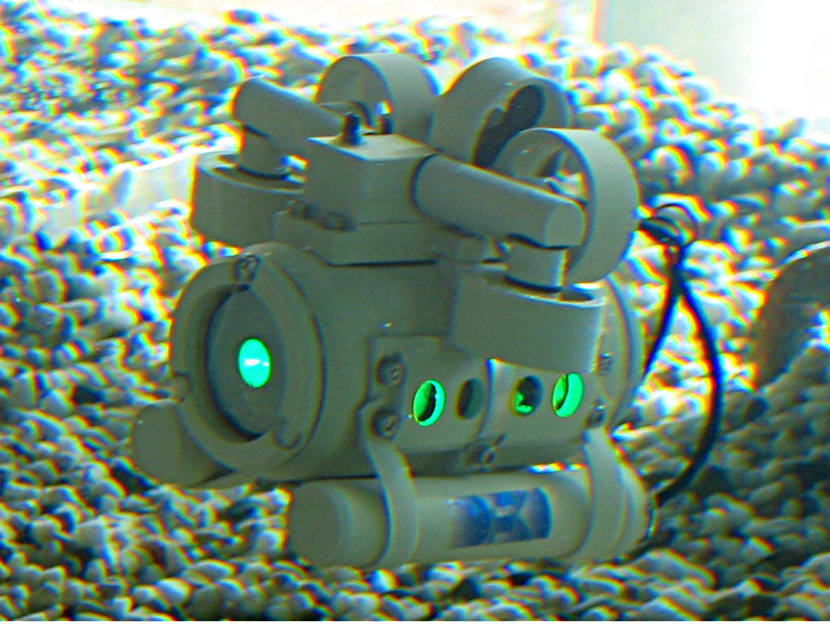
\includegraphics[width=\linewidth]{uauv/uauv.jpg}

\vspace{-1em}
\caption{\scriptsize The \(\mu\)AUV 1~\cite{Fechner2007}.}
\end{figure}
}{0.45}{
\justifying

Vehicle characteristics:
\begin{itemize}
	\item main body diameter of just 55mm and a body length of 125mm
	\item autonomous on-board controller
	\item obstacle detection via active light reflection
	\item depth measurement via pressure sensor
\end{itemize}

\vspace{1em}
Successors: \(\mu\textrm{AUV}^2\) and AUVx.
}

\vspace{-1em}

\begin{center}
\rule{2cm}{0.4pt}\\[0.5em]
\end{center}

\fc{Fechner2007}{publications/2007-02/2007-02}\\[1em]
\fc{Albiez2007}{publications/2007-05/2007-05}

\end{frame}
